\mode<presentation>
{
  \usetheme{CambridgeUS}
  \usecolortheme{whale}
  \usecolortheme{lily}

  \setbeamercovered{transparent}
  \usefonttheme[onlymath]{serif}
}

\title[\BodeControlDesignIShortName] % (optional, use only with long paper titles)
{\course: \BodeControlDesignIName\license}

\subtitle
{Lecture \BodeControlDesignINumber} % (optional)



\begin{document}

\begin{frame}
  \titlepage
\end{frame}

\mode<article>{
\maketitle
\tableofcontents
}

%\mode<presentation>{
%\begin{frame}{Outline}
%  \tableofcontents
%  % You might wish to add the option [pausesections]
%\end{frame}}

\section{Frequency Domain Specifications}

Previously we saw how to translate time domain specifications to frequency domain specifications for a unity gain feedback system

\begin{frame}{Transient Response Specifications}
\begin{center}
	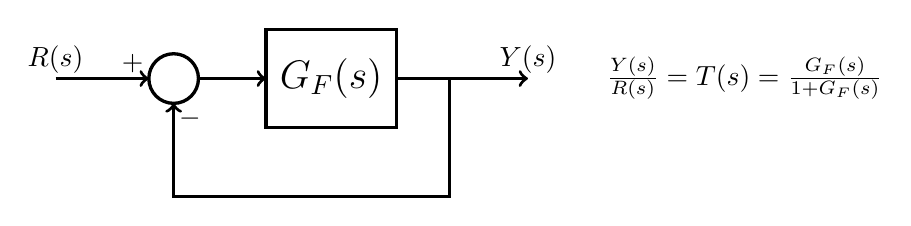
\begin{tikzpicture}[scale=1,inner sep=0pt,outer sep=0pt,very thick,
sysblock/.style={draw,rectangle,inner sep=5pt,minimum width=1.5cm,minimum height=1.25cm,very thick}]
\draw (2,0) node[draw,circle] (sum1) {$\rule{0pt}{18pt}$};
\draw (4,0) node[sysblock] (G) {\Large $G_F(s)$};
\draw[->] (0.5,0) node[above=2pt] {$R(s)$} -- (sum1.180) node[above left=2pt] {$+$};
\draw[->] (sum1.0) --  (G);
\draw[->] (G) -- ++(2.5,0) node[above=2pt] {$Y(s)$};
\draw[->] (G) ++(1.5,0) -- ++(0,-1.5) -| (sum1.-90) node[below right=2pt] {$-$};
\draw (7.5,0) node[right] {$\frac{Y(s)}{R(s)} = T(s) = \frac{G_F(s)}{1+G_F(s)}$};
\end{tikzpicture}

\end{center}
\end{frame}

\begin{frame}
\begin{center}
\begin{tabular}{c|c}
	Closed Loop Step Response & \begin{minipage}{2in}\centering Requirements on Open Loop Frequency $G_F(j\omega)$ \end{minipage}\\\hline
	\begin{minipage}{2in}
		\begin{center}
			\rule{0pt}{14pt}$\OS = \OSeq$\\<all>
			settling time $\ts=\tseqtwo$\\<all>
			rise time $\tr=\treqtwo$\\<all>
		\end{center}
	\end{minipage}
	&
	\begin{minipage}{2in}
		\begin{center}
			Crossover frequency $\omega_{co,G}\approx \omega_{n}$\\<all>
			Phase margin $\PM_{,G}\approx100\zeta$\\<all>
		\end{center}
	\end{minipage}
\end{tabular}
\end{center}
\end{frame}

We can also add requirements on the open loop frequency response due to closed loop steady state error specifications. Recall our investigations of steady state error due to a reference input

%\begin{frame}
%\begin{center}
%\begin{tabular}{c|c|c}
%Reference Command & Steady State Error & \begin{minipage}{1.5in}\centering Open Loop Low Frequency Gain\end{minipage}\\\hline
%Unit Step & $\lim_{t\rightarrow\infty}e(t) = \frac{1}{1+K_{s}}$ & $K_{s} = G(0)$\\
%Unit Ramp  & $\lim_{t\rightarrow\infty}e(t) = \frac{1}{K_{v}}$  & $K_{v} = \lim_{s\rightarrow 0}sG(s)$\\
%\end{tabular}
%\end{center}
%\end{frame}
\begin{frame}
\begin{center}
	\begin{tabular}{c|cc|c}
		& \multicolumn{2}{c|}{Steady State Error to a...} & \textcolor{white}{.} \\
		\mode<article>{
			System Type & Step Input $r(t)=Au(t)$ & Ramp Input $r(t)=A t u(t)$ & Error Constants \\\hline
		}
		\mode<presentation>{	
			System Type & Step Input & Ramp Input & Error Constants \\\hline
		}
		0 & $e_{ss}=\frac{A}{1+K_{s}}$ & $e_{ss}=\infty$ & $K_{s} = \lim_{s\rightarrow 0}G_F(s)=G_F(0)$ \\
		1 & $e_{ss}=0$ & $e_{ss}=\frac{A}{K_{v}}$ & $K_{v} = \lim_{s\rightarrow 0 }sG_F(s)$\\
	\end{tabular}
\end{center}
\end{frame}


These requirements can be summarized in the plot of the ideal {\em open loop} frequency response for $G_F(s)$ for two cases.

\begin{frame}{Open Loop Frequency Response Specifications When $K_{s}=$finite and $K_{v}=0$}
\mode<article>{In the first case (Type 0 system), the magnitude Bode plot has a low-frequency slope of 0~dB/dec, as shown in the figure below. }
\begin{center}
\mode<article>{\input{figures/openloopideal.tex}}
\mode<presentation>{\resizebox{!}{2.5in}{\input{figures/openloopideal.tex}}}
\end{center}
\end{frame}
\noindent For this Type 0 system,  $K_{s} = G_F(0)$ is finite, so when the reference is a step the steady state error is $e_{ss}=\frac{1}{1+K_{s}}$. When the reference is a ramp, the steady state error $e_{ss}=\infty$. 



\begin{frame}{Open Loop Frequency Response Specifications When $K_{s}=\infty$ $K_{v}=$finite}
\mode<article>{In the second case (Type 1) system, the magnitude Bode plot has a low-frequency slope of $-20$dB/dec because of the integrator in $G_F(s)$ (i.e., the term that makes the system Type 1).}
\begin{center}
\mode<article>{\begin{tikzpicture}
\draw (-.25,0) node {\begin{tikzpicture} 
\draw[->,thick] (-.1,0) -- ++(8,0) node[below] {$\omega$};
\draw[->,thick] (0,-.1) -- ++(0,5) node[right] {$20\log|G_F(j\omega)|$};
\draw[dotted] (0,4) node[left] {$20\log(K_{v}/\omega_{\rm low})$} -- (1,4);
\draw[-,rounded corners] (0,4.5)  -- node[circle,fill=black,inner sep=2pt] {} (2,3.5) -- (3,2) -- (5,1) -- (6,0);
%\draw[dotted] (0,1.5) node[left] {$0$ dB} -- (7,1.5);
\draw[dotted] (1,0) node[below] {$\omega_{\rm low}$} -- (1,3.8); 
%\draw[dotted] (4,0) node[below] {$w_{c}$} -- (4,1.5); 
%\draw[->] (4.5,2) node[above] {Slope: -20 dB/dec} -- ++(-.25,-.25); 

\end{tikzpicture}};
\end{tikzpicture}}
\mode<presentation>{\resizebox{!}{2.5in}{\begin{tikzpicture}
\draw (-.25,0) node {\begin{tikzpicture} 
\draw[->,thick] (-.1,0) -- ++(8,0) node[below] {$\omega$};
\draw[->,thick] (0,-.1) -- ++(0,5) node[right] {$20\log|G_F(j\omega)|$};
\draw[dotted] (0,4) node[left] {$20\log(K_{v}/\omega_{\rm low})$} -- (1,4);
\draw[-,rounded corners] (0,4.5)  -- node[circle,fill=black,inner sep=2pt] {} (2,3.5) -- (3,2) -- (5,1) -- (6,0);
%\draw[dotted] (0,1.5) node[left] {$0$ dB} -- (7,1.5);
\draw[dotted] (1,0) node[below] {$\omega_{\rm low}$} -- (1,3.8); 
%\draw[dotted] (4,0) node[below] {$w_{c}$} -- (4,1.5); 
%\draw[->] (4.5,2) node[above] {Slope: -20 dB/dec} -- ++(-.25,-.25); 

\end{tikzpicture}};
\end{tikzpicture}}}
\end{center}
\end{frame}
\noindent In this Type 1 case, $K_{v} = \lim_{s\rightarrow 0} sG_F(0)$ is finite, so when the reference is a step the steady state error is $e_{ss}=0$. When the reference is a ramp, the steady state error is $e_{ss}=\frac{1}{K_v}$. 

The important features of the open loop frequency response are

\begin{itemize}
\item Low frequency gain: either a large gain or a gain that is increasing as $\omega\rightarrow 0$ (i.e., moving from right to left on the magnitude Bode plot) can decrease the steady-state error
\item Crossover at desired bandwidth (with slope of -20dB/dec) to achieve the desired closed-loop natural frequency
\item Phase high at crossover for good phase margin to achieve the desired closed-loop phase margin
\end{itemize}


\section{Analysis of Proportional Control}
One way to design a control system to meet step response specifications is to choose a controller $C(s)$ so that $G_F(s)=C(s)G(s)$ has the desired crossover frequency and phase margin. In this section, we try to do this for the case of a proportional control $C(s)=K$.


Consider the following system: 
\[
G(s)=\frac{5}{s(s+1)(s+10)}
\]%
We would like to design a controller so that the closed-loop, unity feedback system (i.e., our standard configuration) meets these specifications:

\begin{itemize}
\item Zero steady state error to a step input

\item Rise time of  1.1 s

\item $\OS \leq 16.5$\%.
\end{itemize}

The first step is to translate these requirements into the frequency domain. 
It is usually easiest to start with \% overshoot. The required closed loop
damping ratio is found via%
\[
\zeta_T =\frac{-\ln (.165)}{\sqrt{\pi ^{2}+\ln (.165)^{2}}} \geq .50
\]%

The rise-time specification translates to a requirement on $\omega _{n}$
via%
\begin{align*}
\tr &= \treqtwo = 1.1 \\
\omega_{n} &=\frac{2.2}{1.1} = 2
\end{align*}%
Thus the desired $\omega_{n,T}=2$ rad/s. 

Finally, the steady state error specification requires a Type 1 loop gain. Since $G(s)$ already has an integrator, an integrator does not need to be added within the controller, so using proportional control $C(s)=K$ should be adequate.

These requirements on the closed loop poles are then translated to requirements on the loop gain (see Lecture~\TimeFrequencyNumber~for derivations):
\begin{itemize}
\item We can use our approximate relationship $\PM_{,G}=100\times \zeta_T ,$ so the desired phase margin is 50${{}^\circ}$ or greater.
\item We choose $\omega_{co,G} = \omega_{n,T} = 2$ rad/s
\end{itemize}

To examine the design, we will use a control design tool in \textsc{Matlab}. First, let's enter in the system transfer function \\


\noindent \texttt{>> s=tf([1 0],1)\\
>> G= 5/(s*(s+1)*(s+10))}
\vspace{10pt}

\noindent The design tool is initialized by typing \texttt{sisotool} at the command prompt. Depending on which version of Matlab you are using, sisotool may look somewhat different (and is now also called Control System Designer), but the big picture concepts are consistent across most versions. %If you use MATLAB from matlab.mines.edu, it will look as in the notes below. If you use MATLAB in the labs, a primer on the new version, can be found at \url{http://www.mathworks.com/help/control/examples/getting-started-with-the-control-system-designer.html}. However, if you have trouble with this, please use the  matlab.mines.edu.


\noindent \texttt{>> sisotool}

\begin{frame}
\begin{center}
\includegraphics[width=4in]{figures/sisotool1}
\end{center}
\end{frame}

Click on ``System Data'' to load the system transfer function. It opens up the following window

\begin{frame}
\begin{center}
\includegraphics[width=2in]{figures/sisotool2}
\end{center}
\end{frame}

Click on ``Browse ...'' to open up yet another window

\begin{frame}
\begin{center}
\includegraphics[width=3in]{figures/sisotool3}
\end{center}
\end{frame}

Click on ``G'' to choose the transfer function you entered at the command line. Click ``Import'', and ``Close'', and then click on ``OK'' on the System Data window.  In the Control and Estimation Tools Manager window, click on ``Graphical Tuning''. In the row ``Plot 3'', choose ``Plot Type'' as None, so that the window looks like the following:

\begin{frame}
\begin{center}
\includegraphics[width=4in]{figures/sisotool4}
\end{center}
\end{frame}

Click on ``Show Design Plot''. This opens up the window below, where on the left we see the root locus of $G(s)$, and on the right is the frequency response of $G(s)$.


\begin{frame}
\begin{center}
\mode<article>{\includegraphics[width=4in]{figures/sisotool5}}
\mode<presentation>{\includegraphics[height=3.2in]{figures/sisotool5}}
\end{center}
\end{frame}

In the menu of the SISO Design for SISO Task, click on ``Analysis - > Response to Step Command''. This opens the window below. The blue line shows the {\em closed loop} step response, while the green line shows the actuator command (i.e. the signal $u$ which is input to $G(s)$ in the block diagram). This is confirmed by clicking on the plots to see the legend information.

\begin{frame}
\begin{center}
\mode<article>{\includegraphics[width=4in]{figures/sisotool6}}
\mode<presentation>{\includegraphics[height=3.2in]{figures/sisotool6}}
\end{center}
\end{frame}

This step response does not meet our design specifications, because the rise time is greater than 0.9 seconds. This is reflected in the Bode plot, as the crossover frequency is 0.455 rad/s (as seen in phase plot, where it also says that the phase margin is 62.9 degrees) instead of 2 rad/s, where we want it. We can increase the crossover frequency by increasing the gain. This can be done in the SISO Design for SISO Design Task window by placing the cursor over the magnitude Bode plot until a hand appears. At this point, a left click will allow you to grab the magnitude Bode plot and shift it up and down. Shift it up until the crossover frequency is 2 rad/s, as shown in the following figure


\begin{frame}
\begin{center}
\mode<article>{\includegraphics[width=4in]{figures/sisotool7}}
\mode<presentation>{\includegraphics[height=3.2in]{figures/sisotool7}}
\end{center}
\end{frame}

Notice that the crossover frequency is labeled in the \textit{phase Bode plot} (in this image, the text \textsf{Freq:~2.12~rad/sec}) because it's the crossover frequency that is associated with the phase margin $\PM$. 

With this adjustment in the crossover frequency, we can check on the closed loop step response. Right click on the LTI Viewer for SISO Design Task window, select ``Systems'', and de-select the ``Closed loop r to u response''. Then right click again, select ``Characteristics -> Rise Time''. Click on the blue dot that indicates the rise time to get the plot below

\begin{frame}
\begin{center}
\mode<article>{\includegraphics[width=4in]{figures/sisotool8}}
\mode<presentation>{\includegraphics[height=3.2in]{figures/sisotool8}}
\end{center}
\end{frame}

This meets our rise time spec, but now we have a large overshoot! The crossover frequency is 2 rad/second, but since the phase at this frequency is close to $-180^{\circ}$, the phase margin is very low, and the step response is accordingly very oscillatory. This problem can be addressed by using additional terms (poles and/or zeros) in $C(s)$ to alter the crossover frequency without reducing the phase margin, which will be shown in Lecture~\BodeControlDesignIINumber.


\section{Lecture Highlights}
The primary takeaways from this article include
\begin{enumerate}
\setlength{\itemsep}{5pt}
\setlength{\parskip}{0pt}
\setlength{\parsep}{0pt}
\item This article gives an example of designing a proportional controller using frequency response techniques and Matlab's \textit{sisotool}.
\item Please see the Lecture~\TimeFrequencyNumber~for the derivations of the frequency response control techniques used.
\end{enumerate}


%\section{Quiz Yourself}
%
%\subsection{Questions}
%\begin{enumerate}
%\setlength{\itemsep}{5pt}
%\setlength{\parskip}{0pt}
%\setlength{\parsep}{0pt}
%\item \input{quizfigures/quizyourself1.tex} 
%\end{enumerate}
%
%\subsection{Solutions}
%
%\begin{enumerate}
%\setlength{\itemsep}{5pt}
%\setlength{\parskip}{0pt}
%\setlength{\parsep}{0pt}
%\item \rule{0pt}{12pt}\\  % use this \rule command to correctly align solutions given as images
%\begin{center}
%\includegraphics[width=4.5in]{quizfigures/emptyfig.png}
%\end{center}\newpage
%\end{enumerate}
%


\end{document}


